After applying data quality vetoes, there are still noticeable tails in the bulk and edge bin
background distributions that limit the sensitivity of the search. This section aims to identify
the types of instrumental features that are causing triggers with a high re-weighted SNR
and acting as limiting noise sources. This section studies the analysis containing GW150914, which
was detailed in Section \ref{ch:GW150914-DQ}.

\section{Loud transients}

A reasonable hypothesis is that the search is limited by loud transients with an SNR below the
gating threshold. There are certainly a number of loud transients in the data that cause triggers
with very high values of SNR, as seen in Figure \ref{subfig:l1-snr-hist}. It is sensible to check if
the $\chi^{2}$ test down-weights some of these high SNR triggers into the tail of the background
distribution.

To test this, a cut was applied to the CBC triggers to exclude all triggers with an SNR
$>$ 20. The histograms of Livingston re-weighted SNR triggers in Figure \ref{fig:SNR-LT-20-comparison}
show the results of this test.
The green histogram in the foreground of the plot has had all single detector triggers
with an SNR $>$ 20 removed.
The yellow histogram plotted in the background contains all single detector triggers from the analysis.
Any points where the yellow histogram is visible indicate that triggers have been removed by the SNR
cut.
The cut does remove a small number of triggers with  $\hat{\rho} >$ 8, but the overall structure of
the tail is not significantly affected. None of the triggers with $\hat{\rho} >$ 10 are removed by
this cut. Most of the high SNR triggers are down-weighted below $\hat{\rho} =$ 6 and are not visible on
this histogram. A powerful veto that eliminates all CBC triggers
with an SNR $>$ 20 does not significantly improve the tail of the re-weighted SNR distribution.

\begin{figure}[!ht]%
\centering
  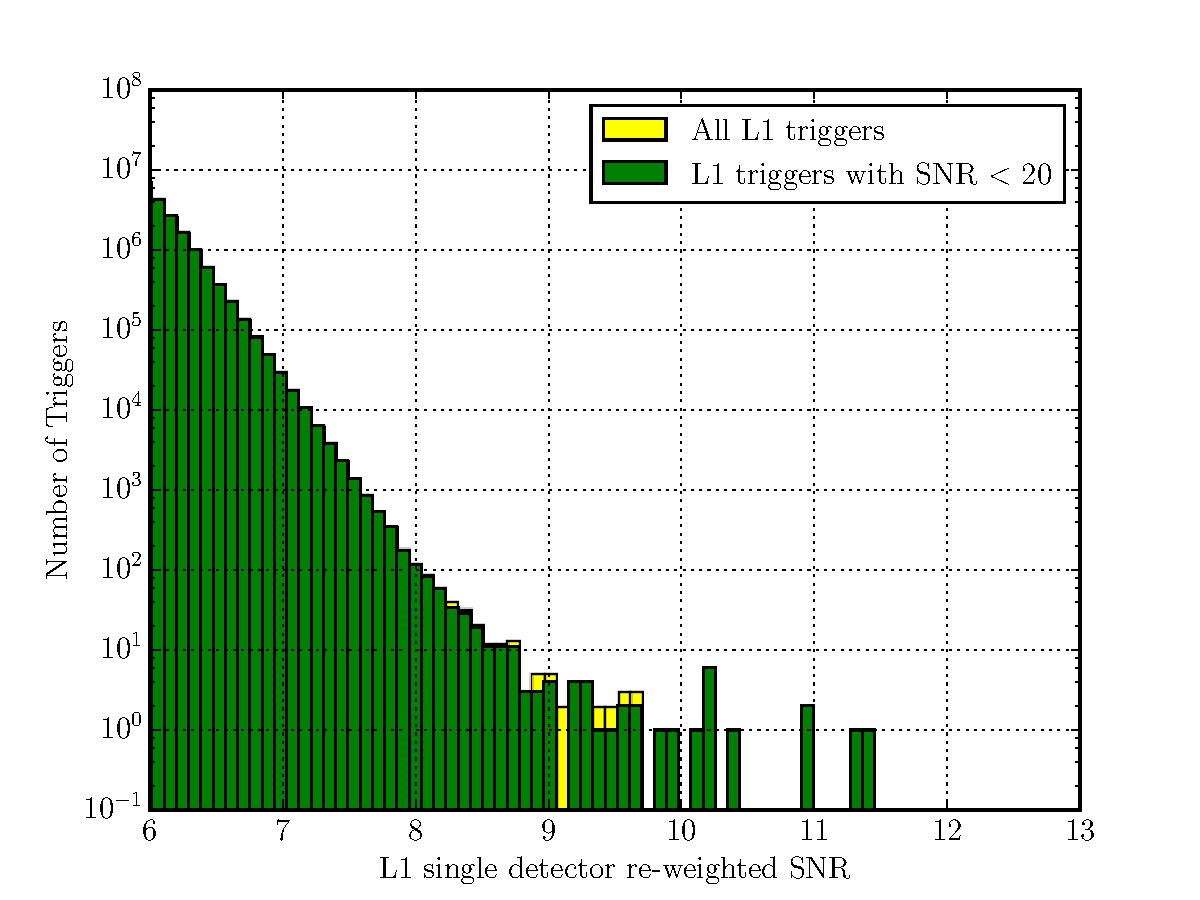
\includegraphics[width=0.9\textwidth]{figures/o1-cbc-dq-paper/L1-newsnr-histogram-compare-SNR-LT-20}
  \caption[Re-weighted SNR histogram with SNR $>$ 20 cut]{A histogram of single detector re-weighted SNR triggers for the Livingston (L1) detector. %
           The green bins indicate triggers %
           with an SNR $<$ 20. The yellow bins indicate all triggers in the data set. %
           The triggers removed by the SNR cut do not significantly impact the loudest events %
           which form a tail in the re-weighted SNR distribution. A small number of triggers %
           at $\hat{\rho} >$ 9 are removed by the SNR cut, but the population is not %
           fully removed. The majority of the distribution is unchanged.}
\label{fig:SNR-LT-20-comparison}
\end{figure}

\section{Blip transients}

The transients that are able to pass the $\chi^{2}$ test and populate the tail in the re-weighted SNR
distribution are in fact those with a specific morphology which resembles that of
certain CBC waveforms. The most common and problematic source of transient noise that causes high
re-weighted SNR triggers are called ``blip transients." These transients are often the source of
the highest re-weighted SNR triggers at both the Livingston and Hanford interferometers.
Although blip transients are seen in both interferometers, they are not found as coincident
triggers and do not represent gravitational wave signals.

Blip transients show up as short duration, band-limited impulses that
have power in the $\sim$30-300 Hz frequency range (see Figure \ref{fig:Blip-omega}).
They don't couple
into any auxiliary channels that are used to monitor interferometer performance. Blip
transient aren't particularly loud, often
recovered by Omicron with an SNR of 10-100, well below the gating threshold applied in the
PyCBC search.

\begin{figure}[!ht]%
\centering
  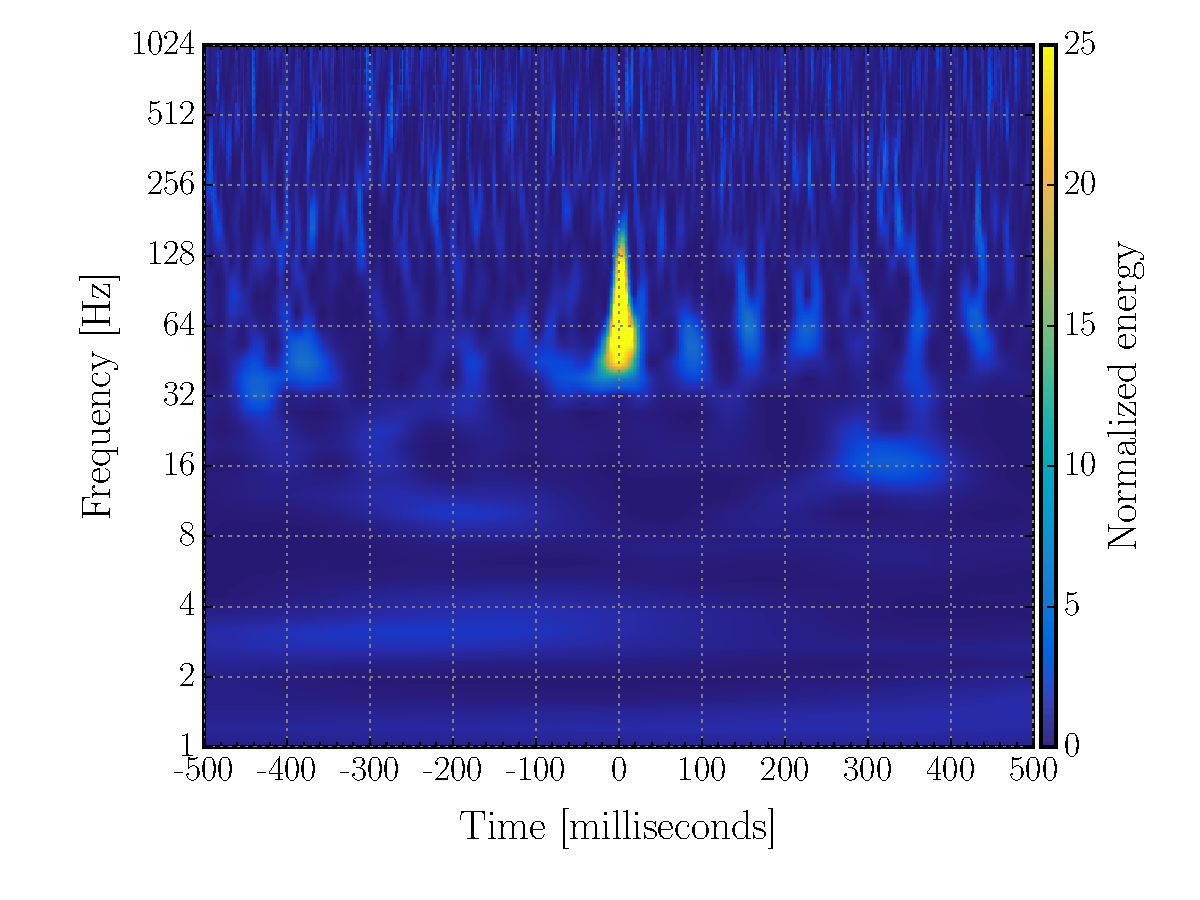
\includegraphics[width=0.75\textwidth]{figures/o1-cbc-dq-paper/Blip-omega-scan}
  \caption[Time-frequency plot blip transient]{A time-frequency representation \cite{ref:omegagrams} of the Livingston strain channel %
           at the time of a blip transient. %
           This visualization of a blip transient demonstrates their typical %
           features: band-limited, short duration, very little visible frequency structure.}
\label{fig:Blip-omega}
\end{figure}

A time-domain analysis reveals
why these are so damaging to the CBC searches. Figure \ref{fig:Blip-cbc-waveform} shows a
filtered time-domain representation of a blip transient in the Livingston strain channel.
The data have been filtered with a bandpass filter
with notch filters to attenuate strong lines in the strain spectrum, double-passed
to be zero-phase. Overlaid on top of the strain data is a CBC waveform that reported a high
re-weighted SNR value at the time of the blip transient under study. The two curves show significant overlap in
the few cycles where the template has appreciable amplitude.

The CBC template that
reported a high re-weighted SNR when filtered against the blip transient in Figure \ref{fig:Blip-cbc-waveform} represents
a neutron star-black hole binary system with a total mass ($M_{total}$) of $98.34 M_{\odot}$ and a
highly anti-aligned effective spin of $-0.97$, resulting in a very short template duration.
This
system will coalesce very quickly and at a relatively low frequency compared to a lower mass
binary system. The waveform
spends less than 0.1 seconds at the frequencies that aLIGO is sensitive to, which,
as shown in Figure \ref{fig:Blip-cbc-waveform}, is the approximate time scale of some
instrumental transients. This time scale is in stark contrast to that of a binary neutron star
waveform, which can have a duration on the order of 1 minute and contain ample signal for use
in the $\chi^{2}$ test.

\begin{figure}[!ht]%
\centering
  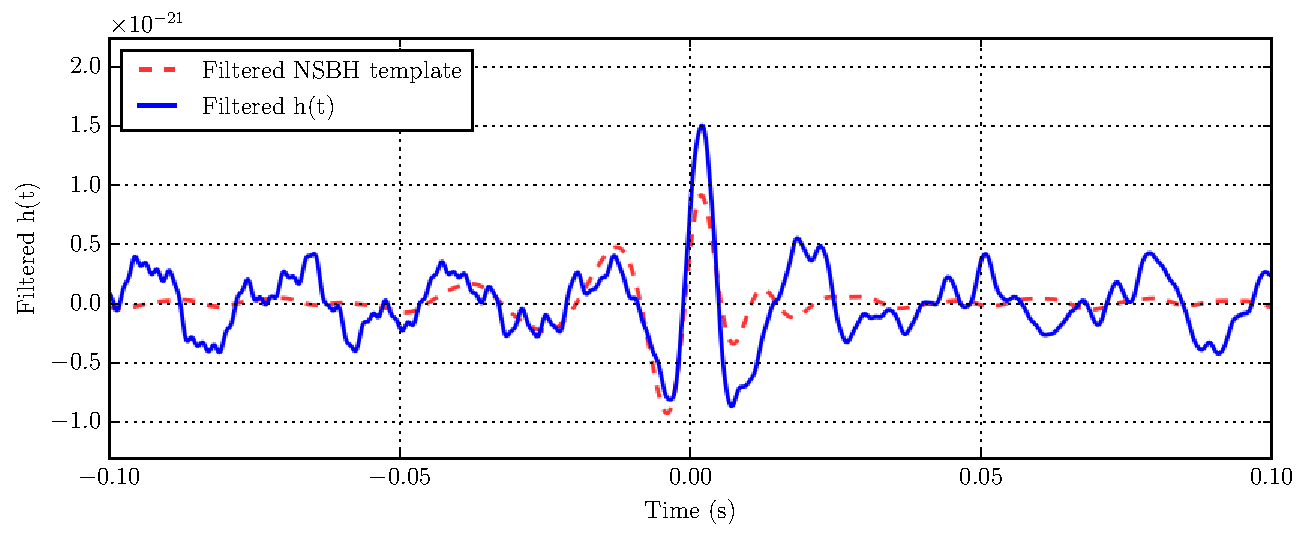
\includegraphics[width=\textwidth]{figures/o1-cbc-dq-paper/Blip-cbc-waveform}
  \caption[Time-series plot of blip transient]{A filtered time-domain representation of the Livingston strain channel, h(t), at %
           the time of a blip transient. Overlaid on the strain plot is a filtered CBC waveform that reported %
           a high re-weighted SNR value at the time of the blip transient. Both sets of data %
           have been zero-phase bandpass filtered to isolate the frequency range that aLIGO %
           is sensitive to. %
           The two curves show significant overlap %
           in the few cycles where the template has appreciable amplitude. The similarity between %
           these two curves causes the $\chi^{2}$ test to be ineffective at down-weighting these transients.}
\label{fig:Blip-cbc-waveform}
\end{figure}

Although blip transients are capable of creating high re-weighted SNR triggers, their effects are
constrained to a fairly small region of the CBC parameter space.
Figure \ref{fig:mtotal-eff-spin-hex} shows single interferometer
triggers from Livingston binned by total mass and effective spin.
The bottom right corner of the plot, bounded by $M_{total} > 80 M_{\odot}$ and
$\chi_{eff} < -0.5$, contains all of the shortest duration templates and the highest
re-weighted SNR triggers. This represents a small fraction of the CBC parameter
space, containing only 65 waveform templates out of 249077 total.
The very loudest triggers in the plot are even further constrained,
corresponding to waveform parameters similar to those in Figure \ref{fig:Blip-cbc-waveform}.

\begin{figure}[!ht]%
\centering
  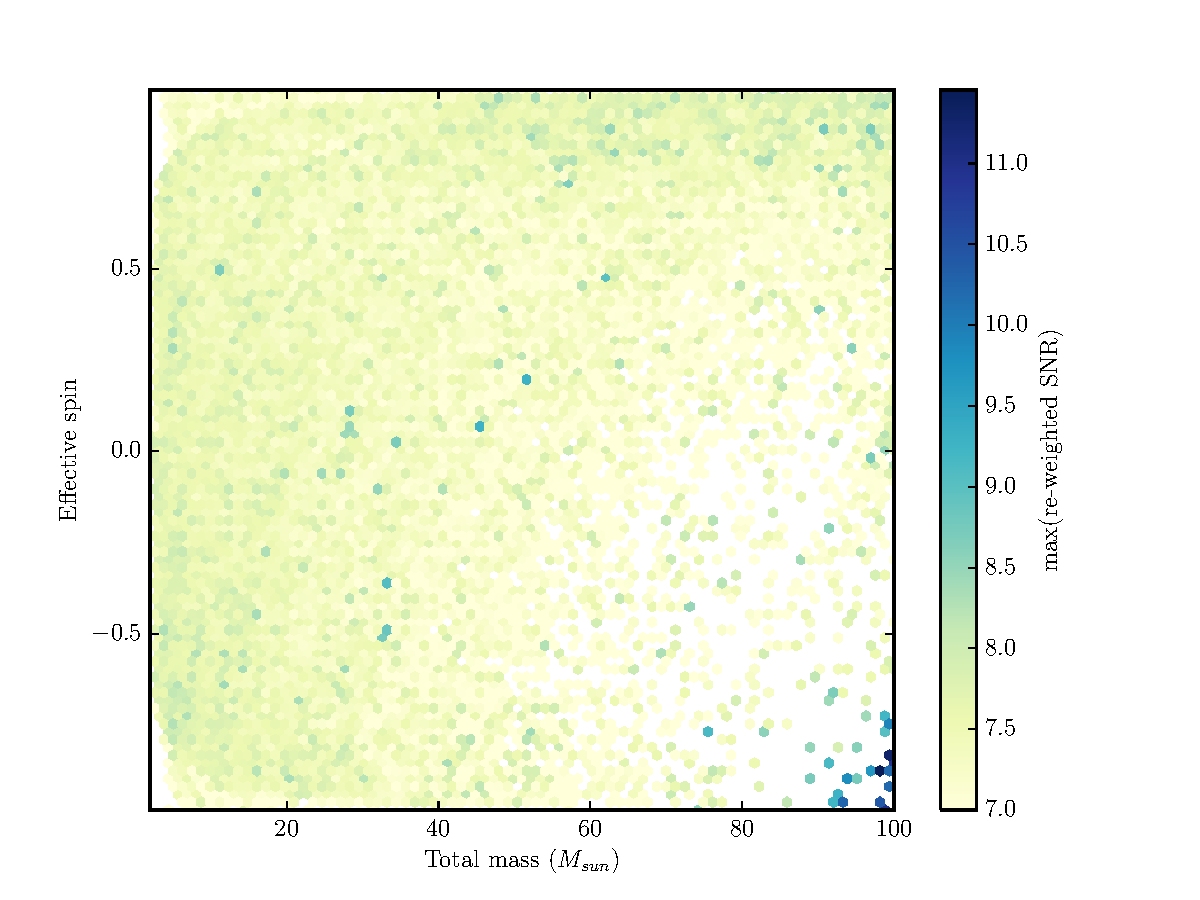
\includegraphics[width=\textwidth]{figures/o1-cbc-dq-paper/mtotal-eff-spin-hex}
  \caption[Total mass vs. effective spin in GW150914 analysis]{A plot of single interferometer triggers from the Livingston detector binned by total mass  %
          and effective spin. The color of each bin indicates the highest re-weighted SNR trigger found in that %
          bin. The highest re-weighted SNR triggers are constrained to the bottom corner of the plot, bounded by %
          $M_{total} > 80$ and $\chi_{eff} < -0.5$. This corner contains the shortest duration templates and %
          is susceptible to instrumental transients such as blip transients.}
\label{fig:mtotal-eff-spin-hex}
\end{figure}

A further investigation reinforces the notion that the loudest triggers correspond to the
templates with the shortest duration. Figure \ref{fig:fpeak-template-duration-hex}
shows single interferometer triggers from Livingston as a function of template duration
and peak frequency of the CBC template. There is a systematic clustering of loud triggers below
a template duration of 0.1 seconds, which is the timescale of typical instrumental transients.
Constraining the loudest triggers using the peak frequency of the waveform template is not as successful.
While the region corresponding to $f_{peak} < $100 Hz does include the templates that are most
susceptible to instrumental transients, it also includes numerous templates with a duration
between 0.1 - 1.0 seconds that do not report any triggers with a high re-weighted SNR.

\begin{figure}[!ht]%
\centering
 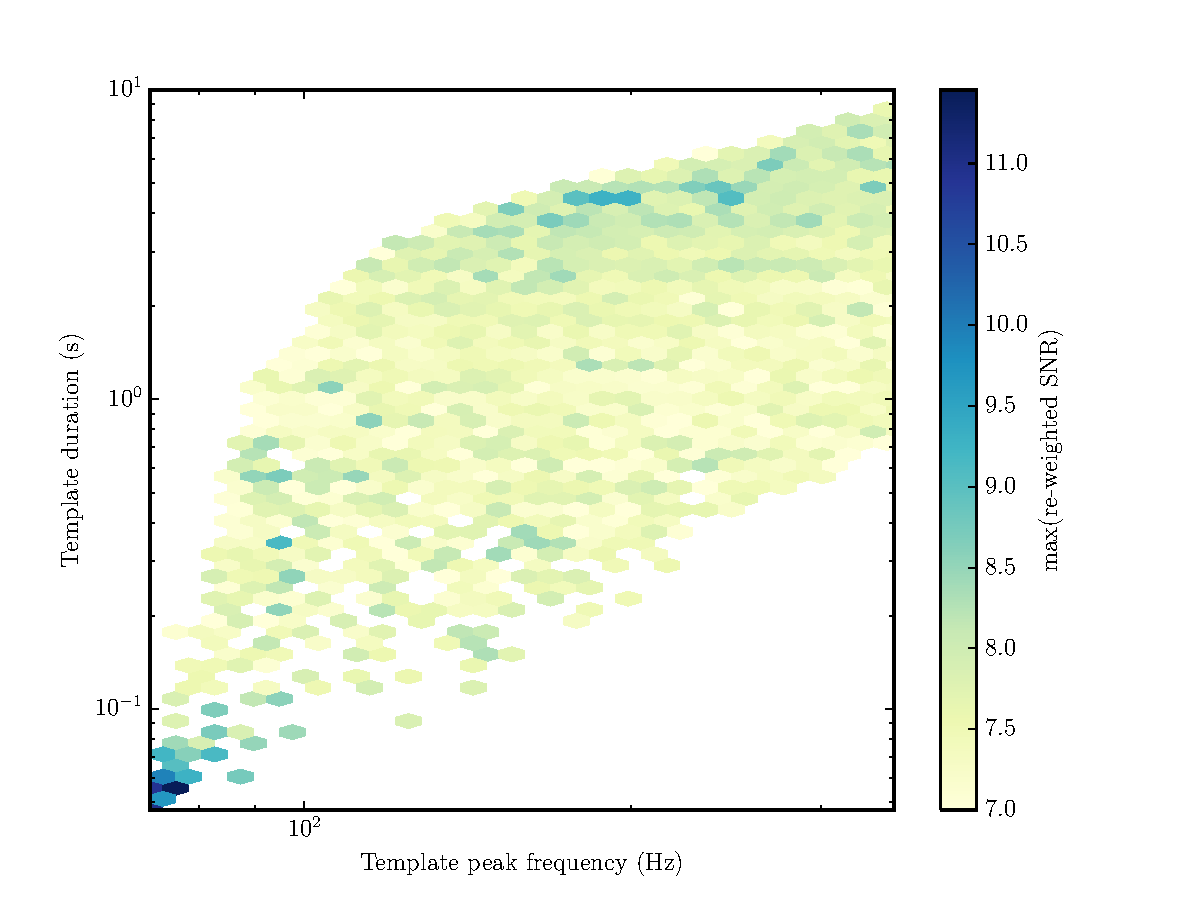
\includegraphics[width=\textwidth]{figures/o1-cbc-dq-paper/fpeak-template-duration-hex}
 \caption[Template duration vs. peak frequency in GW150914 analysis]{A plot of single interferometer triggers from the Livingston detector binned by template %
          duration and waveform template peak frequency. The loudest triggers in re-weighted SNR are %
          constrained to the area of the parameter space with template durations $<$ 0.1s, %
          which is the timescale of typical instrumental transients, most notably blip transients. %
          The small cluster of loud triggers with a template duration of roughly 4.4 s corresponds to %
          the 60-200 Hz noise discussed in Section \ref{sec:60-200-hz-noise}.}
\label{fig:fpeak-template-duration-hex}
\end{figure}

\section{60-200 Hz noise}\label{sec:60-200-hz-noise}

Another limiting noise source for the CBC search is present only at Livingston and
has commonly been referred to as the ``60-200 Hz'' noise. This noise occurs in storms that can
last multiple minutes and are typically comprised of a series of individual flares of noise that
seem to last about 10-100 seconds each. These storms of noise correlate visibly with dips in the
inspiral range, a figure of merit for the CBC searches that estimates the effective range at which
detection of a binary neutron star inspiral is possible based on the shape of the noise curve.
This noise contributes to the tail of loudest background triggers in the PyCBC search, including
the cluster of loud triggers with a template duration of 4.4 s in Figure \ref{fig:fpeak-template-duration-hex}.
Figure
\ref{fig:60-200-Hz-noise} shows the time-frequency representation of this noise on a 20 minute timescale.

\begin{figure}[!ht]%
\centering
  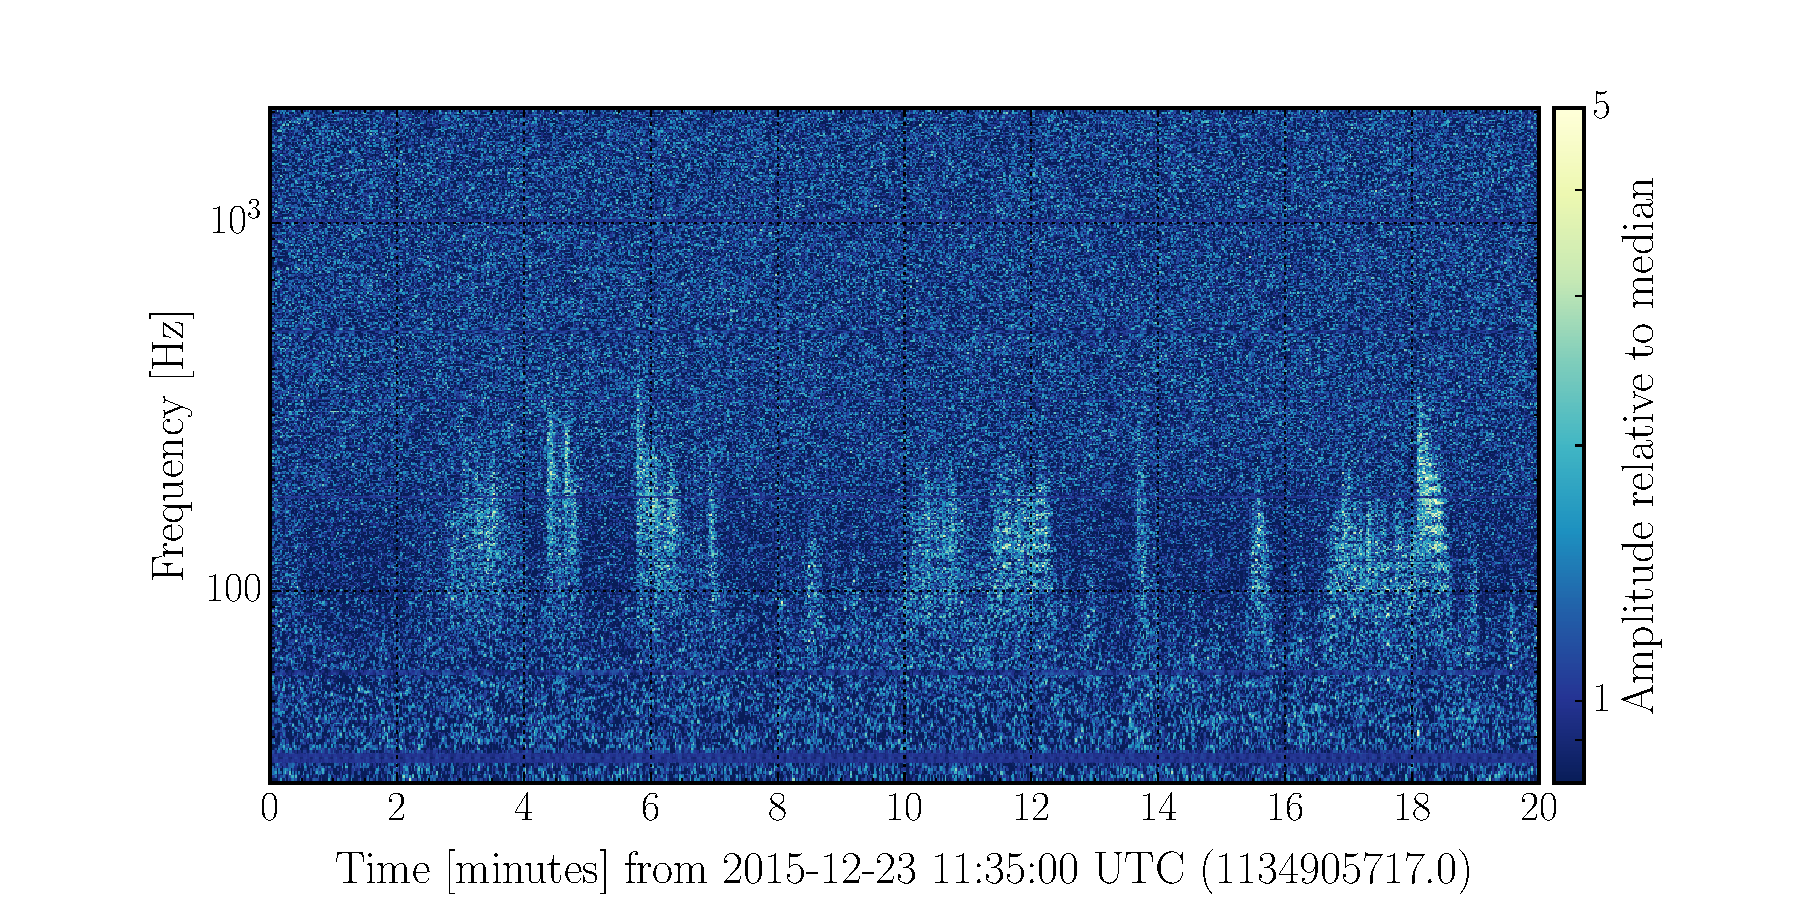
\includegraphics[width=\textwidth]{figures/o1-cbc-dq-paper/60-200Hz-noise-spectrogram}
  \caption[Time-frequency plot of 60-200 Hz noise]{A time-frequency spectrogram of the 60-200 Hz noise. This noise appears in storms %
           that often last for many minutes. This time scale and frequency range is damaging %
           to CBC searches and has often been found responsible for loud background events.}
\label{fig:60-200-Hz-noise}
\end{figure}

A more focused look at these noisy periods
reveals a structure that is reminiscent of scattered light, appearing as arc-like
traces in the time-frequency plane as seen in Figure \ref{fig:zoom-60-200-Hz-noise}. However, the frequency
of this noise is higher than is typically expected from scattered light and investigations have not
been able to find an associated source of scattered light during these noisy periods.
This noise was a common source of high re-weighted SNR triggers in the Livingston
data throughout the first observing run, second only to blip transients.

\begin{figure}[!ht]%
\centering
  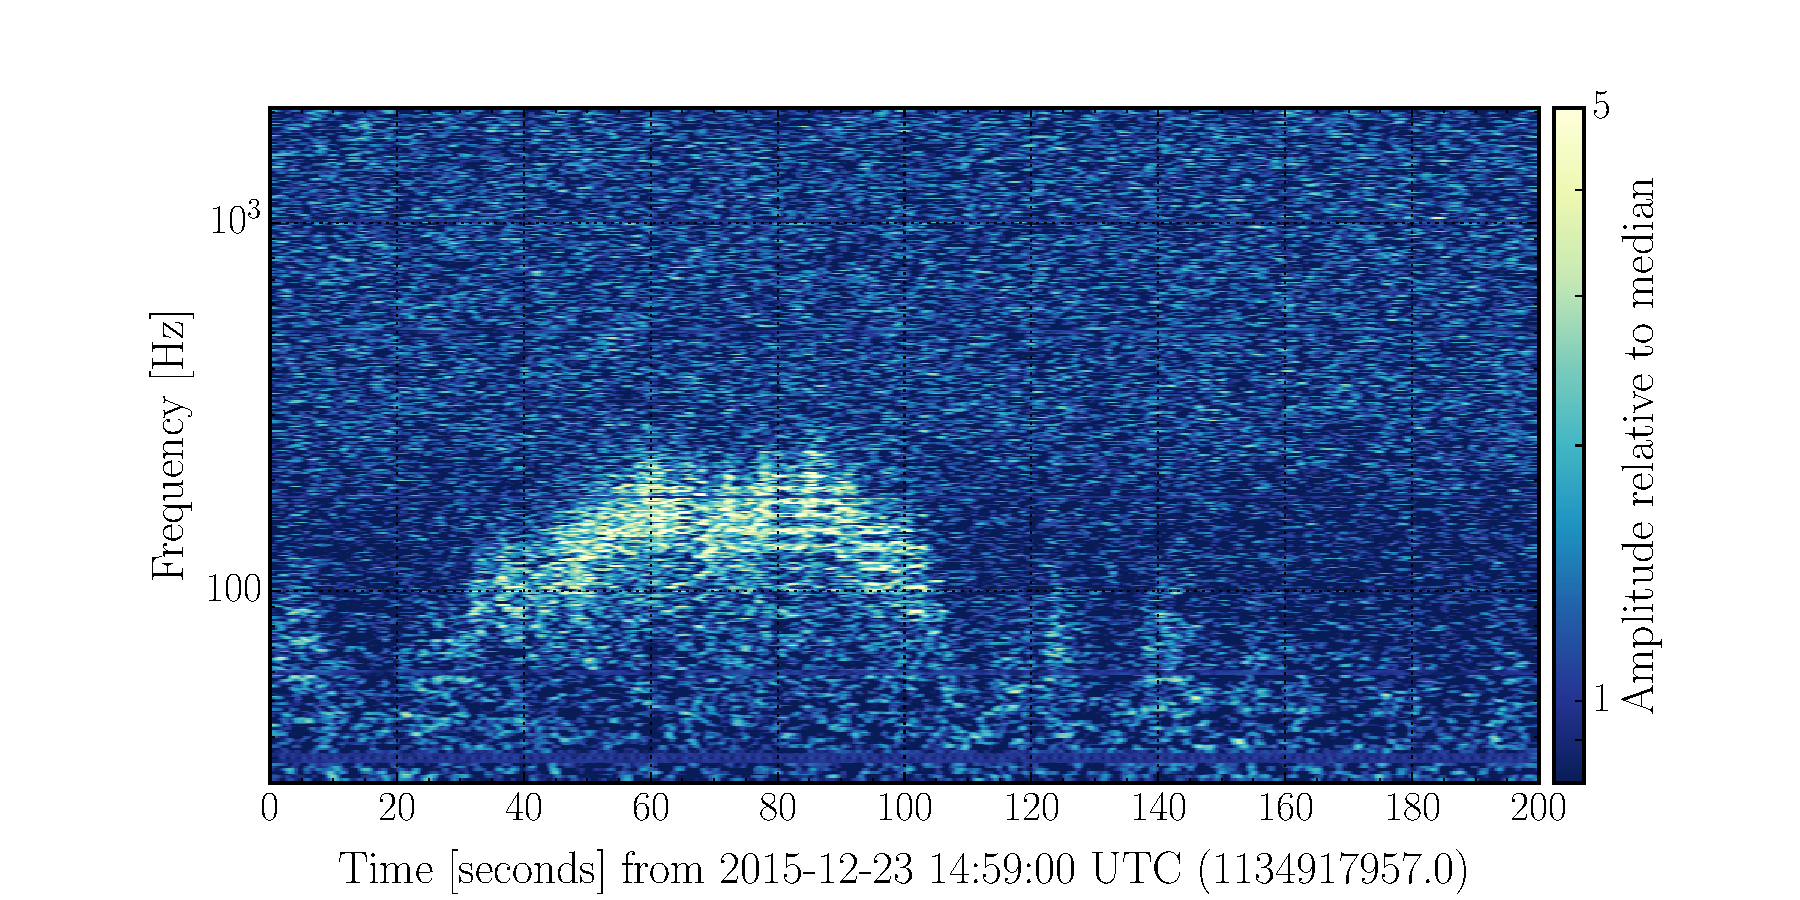
\includegraphics[width=\textwidth]{figures/o1-cbc-dq-paper/zoom-60-200-Hz-spectrogram}
  \caption[Zoomed in time-frequency plot of 60-200 Hz noise]{A zoomed in time-frequency spectrogram of the 60-200 Hz noise. This %
           period of noise caused a loud trigger in the PyCBC background. The %
           arc-like shape of the noise is reminiscient of noise due to scattered %
           light, but the frequency of the noise is higher than expected.}
\label{fig:zoom-60-200-Hz-noise}
\end{figure}
